\chapter{仿真证据的可信度、对照实验与复现方法}
\label{ch:evidence-method}
本章把“仿真成功”拆解为可以独立检查的工程命题。前面的证据图展示现有结果；这里解释为什么选择这些测试、每张图能排除什么错误，以及哪些结论还不能从它推出。所有数字仿真图与模拟电路波形分开标注，生成图形本身不构成通过判定。

\section{从需求到判据的四层关系}
第一层是目标，例如支持一个配置 epoch 下的 16 拍采样间隔。第二层是实现契约，例如采样捕获在哪一个沿发生、转换截止时如何取消、后级结果使用哪个 ID。第三层是激励，例如在第 \(k\) 次 SAR 判决时撤销 valid。第四层是独立判据，例如本帧不提交、下一帧恢复、恢复结果的物理选择和 ID 均正确。省掉中间两层，很容易得到只会打印 PASS 的测试台。

一个完整记录至少包含：源文件 SHA、参数镜像、工具版本、命令行、随机种子或向量文件 SHA、编译退出状态、运行退出状态、完成标记和错误计数。若命令缺失、编译超时或日志来自旧文件，即使目录里还有上一轮 PASS，也必须失败。现有独立算术 runner 对缺工具和陈旧日志有负控；Vivado runner 则进一步要求工件完整、status 与报告条件一致，并拒绝已发现的无驱动综合告警。

\begin{table}[htbp]\centering\small
\begin{tabularx}{\textwidth}{p{25mm}X X}\toprule
层级&有用问题&不能替代的下一层\\\midrule
行为模型&架构关系、误差项与算法是否自洽？&不证明 RTL 的位宽、握手和综合语义。\\
RTL 仿真&整数码、异常与样本协议是否匹配？&不证明工具映射后逻辑仍完整。\\
综合网表功能&关键输入确实影响输出，映射函数正确？&不证明布局布线后达到时钟和功耗目标。\\
实现后 STA/仿真&指定 FPGA、约束和时序角是否收敛？&不证明目标 ASIC 工艺及模拟电路指标。\\
混合信号/PVT&模拟建立、比较器、参考与数字共同工作？&不等于制造后硅片测量。\\
\bottomrule\end{tabularx}
\caption{证据层级及不可越过的推论边界。}
\end{table}

\section{正确值测试与负控测试的区别}
正常值测试回答“已知场景下输出是否正确”。负控测试有意引入一个确定错误，回答“当前测试是否真的能区分这个错误”。如果把最小负值的合法下界写错后，原测试仍全部通过，就不能称它覆盖了有符号边界。

本轮算术负控改变合法最小负值判定和除法位组顺序；结构协议负控恢复旧的组合相位译码或单独恢复旧取消信号。故障均在独立变异副本中注入，生产 RTL 不被污染。应保存变异补丁、命令、预期失败位置和实际失败日志。只记录“负控失败”不足以说明它因目标故障失败，也可能是编译语法损坏；因此需要定位到可解释的断言或逐笔失配。

综合完整性需要类似的负控。基线实际暴露的 \code{Synth 8-3848} 不是人为选择的测试错误，而是真实工具风险；门禁测试应在模拟日志中插入同一告警格式，确认即使工具 raw return code 为 0、status 文件齐全，最终评审状态仍被拒绝。正常无关 warning 则不能被一概当成失败，以免用户学会忽略整套门禁。

\subsection{为什么使用两个独立参考层}
对完整系统，参考模型需要重用物理参数定义才能保持接口一致；但若 oracle 与被测实现复制了同一段位操作，错误也会一起复制。独立任意精度 oracle 从数学定义计算，不导入 RTL 镜像表达式，用来检验乘加、解码和 floor。系统测试再用真实地址/配置/时序驱动完整链路，用来检验集成。

两者互相补足：独立算术不能发现系数写错物理地址，系统斜坡也可能看不到最小负数边界。所谓独立并不是完全没有共享任何常量；正确做法是公开哪些输入定义共享、哪些运算实现独立，以及生成器是否调用了被测公式。

\section{各类图怎样读取才不误判}
\subsection{码值与差值}
上层图可画实际码和期望码，便于观察范围、单调性和样本缺失；下层必须画差值或逐笔错误标记，因为百万级码范围会把一个 LSB 的失配掩盖。通过判据来自全部原始样本的整数比较，图中抽样用于显示，不能反过来用稀疏像素证明全数据一致。

横轴应注明是 DUT sample ID、测试台序号还是时间。兼容顶层 P3 的图来自测试台计数，其 DUT ID/flags 端口未接，不能作为跨样本 ID 正确的证据。结构协议与拟合留出测试则显式检查 ID。即使两张图横轴都写“sample”，其证明能力也不同。

\subsection{误差改善图}
校准恢复夹具的最大误差从名义权重的 504 码降为 4 码，说明对所注入的固定合成失配，载入系数和整数校正有明显效果。这不是 SNDR、ENOB 或 INL 的等价表述。要计算 ENOB，需要明确频率、幅度、采样率、长度、窗函数和噪声/失真处理；要计算静态 INL/DNL，则需要转移特性或规定的码密度实验。把误差改善比直接取对数写成动态范围会混淆量纲和测量定义。

\subsection{延迟和协议波形}
延迟以接受 start 的有效沿为零点，而不是以驱动器试图发 start 的时刻为零点。busy 期间的 start 被拒绝时，不应计入成功事务。完成边沿和下一次启动边沿可能不同；因而同时记录结果延迟、busy 释放时刻和可接受下一样本的间隔。

P5/P6/P7 的 15/13/11 拍重构延迟由两个范围不同的夹具核对。最新精简权重 RTL 已在 \code{ci_rtl_0c4a/} 的连续启动夹具中对每档重跑32笔、间隔16拍的请求，检查无合法样本丢失及 busy 在14/12/10拍释放。该夹具使用缩小阵列。\code{compact_profiles/} 另运行生产18-slice结构顶层：每档检查438次输出、438次精确延迟和7,680个协议节拍，三档仍分别得到15/13/11拍。两项均有当前内容摘要对应的实际日志；旧 \code{final_profiles/} 仅作历史归档保留。

这些是 RTL 协议和功能仿真的拍数，不能证明实际 FPGA 的每一拍都能做到约 1.563 ns。仿真中的时钟周期是激励条件，只有加入正确的延迟模型并满足实现时序后，才能把它与物理频率联系起来。

\section{覆盖矩阵的实质内容}
覆盖矩阵应围绕故障机制组织，不能只按文件名列出“已测”。例如，采样注入符号、主子组权重排列和负数 floor 都会影响最终码，但需要不同激励才能区分。下面给出本工程已有测试与应继续补足的关系。

\small
\begin{longtable}{>{\raggedright\arraybackslash}p{29mm}>{\raggedright\arraybackslash}p{47mm}>{\raggedright\arraybackslash}p{70mm}}
\toprule 故障机制&已有区分证据&仍需保留的边界\\\midrule\endfirsthead
\toprule 故障机制&已有区分证据&仍需保留的边界\\\midrule\endhead
正负号/隐式宽度&90,058 向量的独立整数对照与边界负控&有限测试不是对全部 64-bit 输入的形式证明。\\
物理地址错配&1278 项镜像加载、留出事务与物理校准夹具&真实电容版图地址和软件排序还需系统集成核验。\\
错误位晚一笔&定向异常、保持行为和当前 ID 检查&ADC2 告警与硬错误的消费策略需软件遵守。\\
跨相位污染&120 帧丢失 valid/迟到活动/恢复测试&异步模拟比较器的 CDC 和亚稳态不在零延迟 TB 内。\\
归约代数改写&两个 Verilator 版本各 1,430,848 次检查、7 个几何；新旧实现均对照独立 scalar oracle&补强后的判据检出共同错误；RTL 结果仍不能发现特定综合器丢失树。\\
前向引用综合差异&旧网表 warning、常量化及无扇出；两种连接修复见证均通过12904次XSim比较&小单元的输入因果与功能检查不能代替完整顶层的约束和实现验收。\\
除法组合链过深&真实 timing path 的 carry 级与起止寄存器&单独优化除法后，最坏路径可能转移到归约或 MAC。\\
配置并发冲突&完整性 bitmap、clear/validate/写入冲突回归&外部总线跨域协议不是当前同步接口自动提供。\\
\bottomrule\end{longtable}
\normalsize

\section{从波形追查一次失败的标准流程}
出现某笔最终码失配时，先确认其 sample ID 与配置 epoch，再确认 \(F,O,I\) 和 \(T,G,R\) 是否属于同一份快照。如果在这一步就发现物理选择不同，应优先定位上下文捕获和前后级调度，而不是调校算术公式。若输入快照完全一致，再把每一级整数中间值导出给任意精度 oracle，查出第一个不一致的操作。

对边界失败，保留数值的十六进制位型和有符号十进制解释。只看十进制有时会忽略截断位宽，只看十六进制又不容易辨认负数。对时间失败，保留接受沿、deadline、cancel、valid、done 和输出沿；不要只截取最终报错时刻，因为根因可能发生在一个 frame 之前。

综合后失败还需多一层：检查优化日志和输入扇出，确认该输入仍参与目标函数。若某个功能块被综合成常量，先解决 elaboration 或约束问题，再看关键路径。对无驱动节点加 \code{keep} 不会创造本来缺失的驱动；增加 timing exception 更不能恢复逻辑。

\begin{figure}[htbp]\centering
\begin{tikzpicture}[>=Stealth,font=\small,node distance=7mm,b/.style={draw,rounded corners,align=center,text width=120mm,minimum height=10mm}]
\node[b] (i) {失配样本：固定源码 SHA、配置、向量与工具版本};
\node[b,below=of i] (c) {先检查 ID、epoch 和物理开关快照是否属于同一残差};
\node[b,below=of c] (a) {快照一致后，逐级核对 \(T,G,R,F,N,A,q\) 与独立整数 oracle};
\node[b,below=of a] (s) {只在综合网表失败时，检查 elaboration、驱动、扇出和常量传播};
\node[b,below=of s] (t) {功能成立后，再比较 setup/hold、关键路径、布局和功耗};
\draw[->](i)--(c);\draw[->](c)--(a);\draw[->](a)--(s);\draw[->](s)--(t);
\end{tikzpicture}
\caption{按因果顺序定位失配，避免把错误输出归因于尚未测量的模拟噪声。}
\end{figure}

\section{本轮 CI 编译超时与测试失败如何区分}
发布提交 \code{50b5733} 后，RTL CI 在七几何归约 miter 的 Verilator/C++ 编译阶段超过 300 s，尚未进入该 bench 的运行断言。该状态不是功能通过，也不是已经证实算术失败；正确记录是“此运行没有获得结果”。本轮将该大型 bench 的编译限时单独设为 900 s，并把 RTL job 总限时调整为 45 分钟，运行期仍使用单独的有限预算。

这项修复没有减少向量数、屏蔽断言或把超时改成成功。编译日志和运行日志分开保存，先删除旧的 run log，再创建新工件。对于其他普通 bench 仍保留原来的 300 s 编译限时，以便真实卡死及时暴露。旧版修复基线（RTL 内容摘要前缀 \code{169f957dc7fe}）曾在本地完整重跑 21 项 RTL 测试和 3 类 lint，\code{final_rtl/result.json} 记录该轮整体退出码 0 及 21 项完成标记；其中旧版归约 miter 记录全部 1,430,848 次比较。它使用当时的测试台和判据，不包含下节随后加入的独立 scalar 检查，也不能改标为精简权重存储版本的全量重跑。新提交的GitHub CI状态仍须独立确认，不能把本地通过或旧提交的绿色状态贴到新源文件上。

本轮本地全量回归还有一次构建环境失败：make调用的进程PATH里没有Python。该尝试没有有效仿真结果，原失败记录保留；补齐当次进程 PATH 后从旧版冻结源码完整重跑，才形成 \code{final_rtl/} 的历史成功证据。这个例子说明“环境修复”和“算法修复”应分别登记，避免把一次未运行的测试写成曾经算术失败。

\section{两份实现共同错误时，miter 为什么也会漏检}
提交 \code{39e9c27} 的后续 CI 在 Verilator 5.020 上进入实际运行后，
七几何归约 miter 于 \code{NS=32,NM=2,ND=1,DE=3} 的第 13 次检查失败。
这次不再是编译超时，不能沿用前一次故障解释。
用官方 5.020 源码构建的本机工具、原七实例 testbench、相同展开参数和优化级别，
再次观察到同一检查失败。

进一步保留原生成模型，只在相应 C++ 检查前增加诊断打印，发现更重要的现象：
前面的定向用例中，测试台权重已经为 1、8 个物理 slice 已选中，
但两份实现的 \(T\) 与 \(G\) 同时保持 0；独立数学值应为 24。
因此，miter 在首次报错之前已有双方共同偏离正确值的情况。
仅有 \(Y_{\rm new}=Y_{\rm old}\) 不能证明 \(Y_{\rm new}=Y_{\rm correct}\)。
当前工具生成代码把相关总和的赋值放在初始 settle 路径中，未随这类刺激按预期重算；
它是本次具体测试结构与工具组合的证据，不足以泛化为全部 packed-array 写入均有问题。

改进测试台时，保持生产 RTL、七种几何、随机种子、刺激顺序、43,758 种分配
以及全部原始比较不变，在明确的测试时钟沿捕获整包输入，
另一个沿以逐物理单元的 scalar oracle 同时检查新旧结果。
checker 与刺激生成分开，首个有效捕获沿安排在仿真启动之后；
每个几何还校验原有检查数量，避免忽略首样本或提前退出后仍打印完成。
这里只增加 testbench 的事务边界，没有给组合 DUT 增加生产流水级。
最终归档 \code{docs/evidence/20260930/reducer_scheduler/manifest.json} 记录：
修复后的同一测试台在 Verilator 5.020 与 5.49 下分别退出 0，
每次均出现七种几何的完成记录及总完成标记，检查总数各为 1,430,848。
生产尺寸的 43,758 个分配组合包含在上述计数中；两个工具运行同一激励集合，不能相加成更多覆盖。
对应 \code{after_5020.run.log} 与 \code{after_549.run.log} 保存原始结果，
被测归约器内容摘要前缀均为 \code{c5fc7f6ef58b}，也与 compact 版本一致。

共同错误负控只把两份实现共享的权重快照清零，保持原始刺激及 scalar oracle 不变。
5.020 运行在第 9 个检查点报参考值失配并以 134 退出：正确的 \(T,G,R\) 均为 24，
两份实现却均为 0。它说明新判据能识别原 miter 会接受的“双方同错”，
不把断言预期失败当作工具崩溃或成功仿真。
图\ref{fig:reducer-scheduler-evidence} 展示日志实际保留的前 16 个检查点及该负控，
原始失败日志与 printf-only 诊断副本一并保留，未覆盖历史运行。

\begin{figure}[htbp]
  \centering
  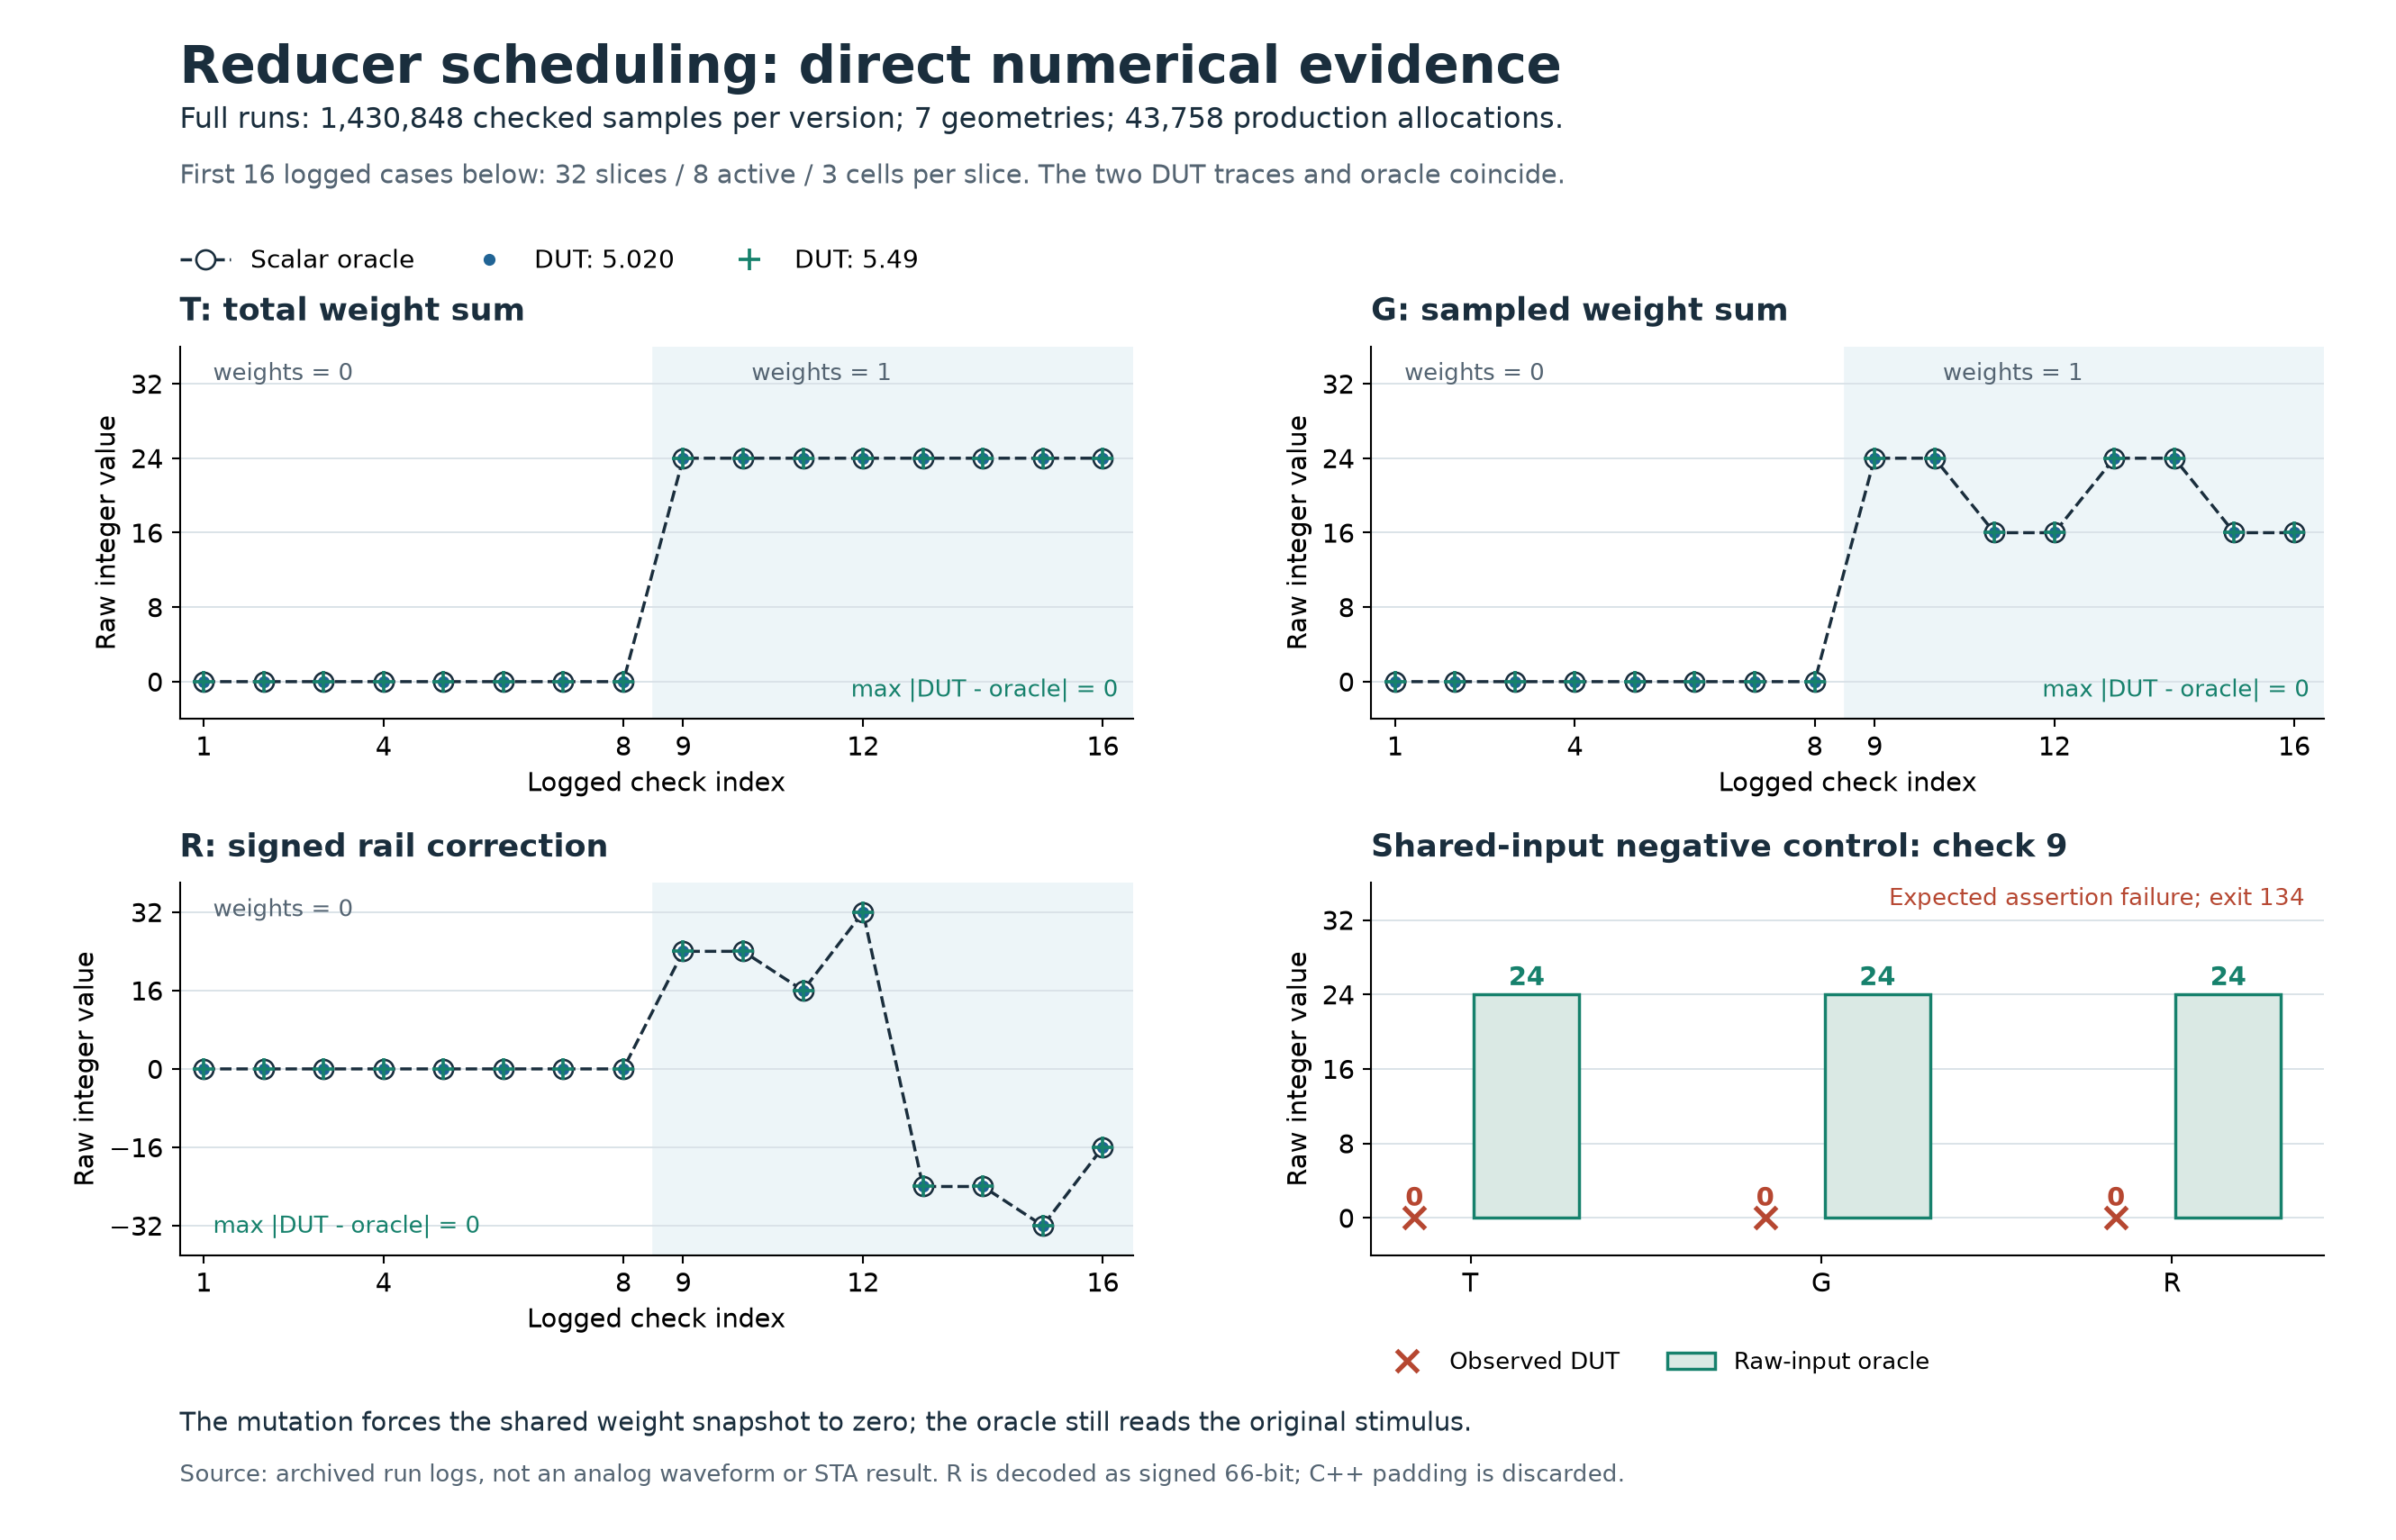
\includegraphics[width=\textwidth]{figures/39_reducer_scheduler.png}
  \caption{归约验证中的数值证据与共同错误负对照。前三个面板仅绘制32个物理slice、8个活动slice、每slice含3个单元这一配置的前16个日志检查点；两个工具版本的DUT结果与逐物理单元的独立参考在这些点重合。完整回归在每个工具版本下分别检查1,430,848个样本，覆盖7种几何配置及43,758个生产分配组合，不能把两次工具运行的数量相加当作额外覆盖。右下角将双方共用的权重快照故意清零，原始刺激参考仍为24，在第9个检查点被断言检出。横轴是检查序号，图中没有重建模拟波形，也没有给出静态时序结论。}
  \label{fig:reducer-scheduler-evidence}
\end{figure}


\subsection{Python 位级镜像的宽度同步}

同一提交的 Python CI 还正确发现另一类问题：生产除法器的余数宽度已改为
\(W_R=P_{W_A}\)，位级镜像却仍使用 \(\max(P_{W_A},P_{W_D})+1\)。
修复同步了宽度、高位分母分类和 \(W_R+1\) 位借位减法，保留原有反漂移门禁。
新增六种小几何共枚举 55,432 个输入对，包含 308 个零分母、31,744 个高位分母分类用例，
以及最负数、非整除的展开 padding；25 项镜像测试全部通过。
本地非 slow Python 回归执行 \code{PYTHONPATH=$PWD/src python -m pytest -m "not slow" -q}，
日志记录 918 项通过、3 项未被选入，用时 678.00 s。
该次收集之后新增的完整顶层映射流程测试另行验证，不能据此把 918 称为当前全部测试数。
证据位于本地实验目录 \code{sar_adc_vivado_20260930/python_regression/manifest.json}；
其原始日志摘要为 \code{82fad3175aa905eac17a80e78fe4a0f98b74f7fe779808225b75373e913bfc74}。
六个小几何的独立复核及 25 项镜像测试另见同一实验目录的
\code{full_mapped_flow_checks/mirror_independent_review.json}。
镜像用例、Python 测试与 RTL 向量有不同计数单位，也有重叠的回归范围，
不能将它们相加为覆盖率或替代最终 GitHub 提交的 CI 状态。

\section{未来动态性能验证应怎样接入}
数字重构修复完成后，可把真实行为模型或混合信号仿真的连续输出导入 ADC 指标工具。但输入必须含均匀采样时间或明确的缺样记录，且剔除启动阶段的方法事先规定。发生错误但保留旧码的事务不能悄悄当作正常样本送入 FFT；要报告错误率，并明确频谱是否来自仅成功的连续区间。

对每个动态场景，至少保留输入频率/幅度、采样率、样本数、窗函数或相干关系、去直流规则、谐波归类、噪声积分带宽与结果单位。对比校准开关时保持相同输入和模拟失配实现，避免把两次随机噪声差异误判为校准收益。时间交织和 DEM 的周期还会产生特定离散 spur，不能只观察最大谐波附近几个 bin。

静态验证应包括端点处理、单调性、漏码和最大局部步长。对 20-bit 全码域，扫过理想整数输入并得到相同数字输出是一个有用的映射测试，但不等同于用连续模拟输入测出所有真实转换阈值。实际模拟非线性、比较器噪声和建立误差必须出现在刺激到输出的路径中，才能被该实验观察。

\section{交付工件的最小集合}
最终工件按用途保存：源码与约束定义要执行的设计；原始日志与 status 文件记录工具实际行为；manifest 和 SHA 将两者绑定；图和报告解释结果。图的像素文件不应成为唯一证据，因为读者无法从图中复原全部码值和异常序列。对于体积较大的 DCP 或完整波形，可以保留在本地实验目录，并在公开仓库中放哈希、生成命令和精简文本报告。

原始失败工件应保留，后续更正通过独立 reviewed result 说明它为何失效。本轮 Windows Vivado 的外层批处理返回 0，而 Tcl status 明确指出负 WNS；这需要区分 raw return code 与归一后的时序结果。随后发现的无驱动又否定了该网表的功能完整性，因此最终状态必须进一步降级为无效综合诊断样本。按时间覆盖原 manifest 会抹去这条发现链，降低可追溯性。

这套组织方法的目的，是让另一位工程师从提交和命令重新得到相同的通过或失败结论，而不是只相信报告作者的描述。对当前工作，功能等价、综合完整性和时序闭合分别列为独立验收项；任何一项未完成，都不得用另外两项的成功替代。
